\documentclass{article}
\usepackage{graphicx}

\title{Po-Shen Loh: the Traveling Salesman of Mathematics}
\author{Owen Xuan}

\begin{document}

\maketitle
He runs down the hall, talking to himself, but nobody is surprised. Suddenly, he stops. Turns left. An office. His office at Carnegie Mellon University.

Born in Madison, Wisconsin to a family rich with math ideas, now-professor Po-Shen Loh has influenced thousands of young mathematicians in the interesting path of his life. If you took a student from the math forums of Art of Problem Solving (AoPS), nine out of ten times they would recognize his name.  Yet throughout his journey, Loh is humble and remains willing and eager to, in his words, “get his hands dirty and build something.”

Along with many others, I was witness to this “build something” aspect of Loh’s personality. We participated in his daily virtual “Ask Math Anything” streams, which often lasted over an hour, was there at his in-person talk in Seattle, and read with wonder about NOVID- a practical program created with abstract math that goes beyond COVID contact tracing.

“Ask Math Anything” streams were a lighthouse for that era for me. Streams were unorganized, in that the content wasn’t planned, but was reassuring because of their consistency and atmosphere. Viewers formed connections with other strangers from the shared experience of watching someone who truly had a passion for raising the interest of math and changing the way it was learned. (And from insisting that he wore a green shirt!) As each stream started, these viewers would ask their questions, sometimes hitting the core of what it meant to learn math, other times presenting a math problem they found intriguing. Loh would answer these questions, demonstrating a profound capability to dissolve hard problems in easy concepts. April brought the end of the streams. In one of the final AMAs, Loh shared his newest project (viewers knew about it before the U.S. government!): NOVID.
\begin{center}
    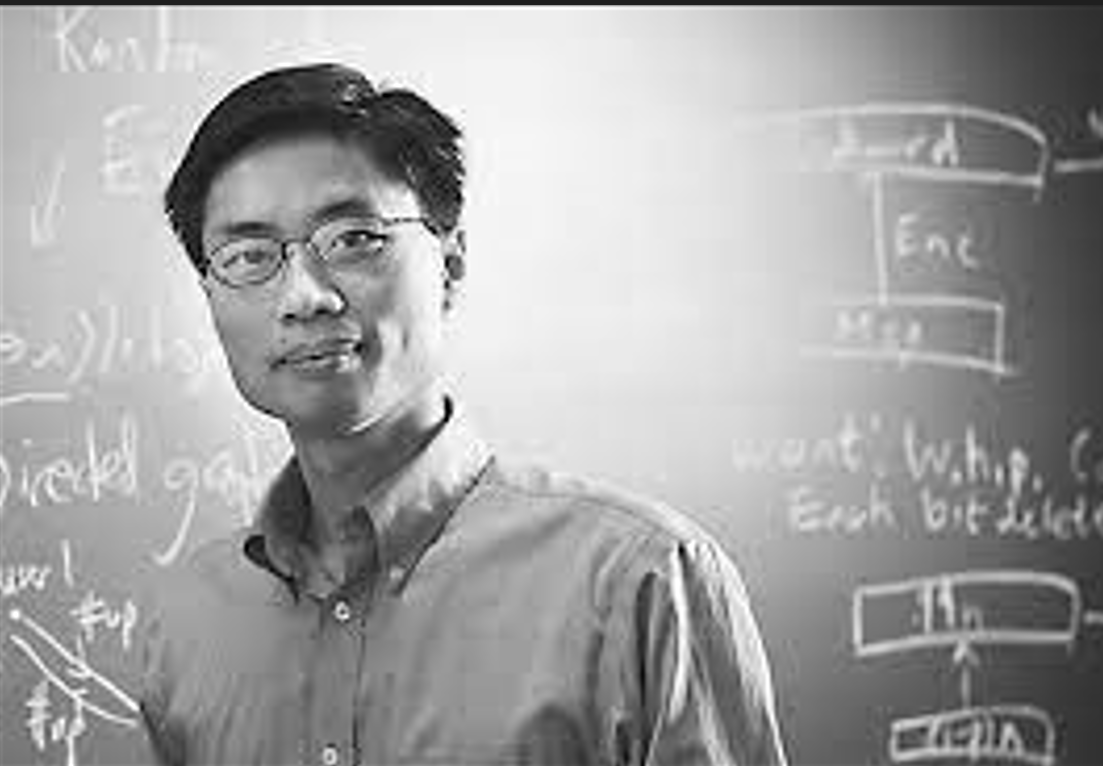
\includegraphics[scale=0.35]{images/po-shen loh.png}
\end{center}

“If you see some task that you’ve never seen before, can you actually invent a new approach to it?” By this quote, we see not only Loh’s focus on inventing-based learning, but a reflection of his values in his work. In a 21-page paper, Loh said the app will “introduce a fundamentally different paradigm for contact tracing”---it’s innovation in the best sense. In essence, Loh had created a type of “6 degrees of Kevin Bacon” for tracking the coronavirus; instead of only alerting a person after exposure, the app used various sensors to notify each person (before exposure) of how many relationship ‘degrees’ an infectious person has from them. If a friend of a friend contracted the virus, that would be two degrees of separation. This type of thinking falls under the umbrella term “network theory”, which was a basis of the envisioning of NOVID in prototype. Now, the app has reached over 100,000 users.

Four months after the streams ended, Loh gave a talk at Seattle, on a stage overlooking a grassy hill. Before the event started, Loh set up the entire stage, microphone, and speakers- with no crew. Later, I would learn that these trips marked the rebooting of his nation-wide tour before the pandemic. As we listened, the “traveling salesman of mathematics,” as Loh refers to himself, described how his combinatorial background applied to games, parties, Ramsey theory and NOVID. He tells us his goal is “to build the world to be a more thinking place.” Later, as it started to drizzle and Loh began to pack up, a few others and I approached Loh to ask questions and talk. He was friendly and willing to answer questions, and left Washington slightly soaked and having inspired dozens. Everything was perfect! Until he tested COVID-positive, with me as his last contact. (I swear it wasn’t me.)

The man running down the hall is Po-Shen Loh. He hurries to try to “milk every second”. Chances are, in that second, he’s thinking about making the world a more thinking place.
\end{document}